\chapter{De los cuantos de cuerda abierta a los taquiones y la gravedad}

\lectureoverview{Ahora cuantizamos los modos normales obtenidos en la clase anterior y preguntamos qué estados de partícula producen. Cada modo transversal es un oscilador armónico, pero su normalización resulta algo poco habitual: excitar el modo \(n\) aumenta la energía de frente de luz y, por tanto, el nivel del cuadrado de la masa, en \(n\) unidades. El primer nivel excitado de la cuerda abierta se transforma exactamente como las dos polarizaciones transversales de un vector sin masa. Por consiguiente, la consistencia relativista fija un valor negativo para el cuadrado de la masa del estado fundamental. Ese estado es el taquión de la cuerda bosónica, cuyo significado real es que el vacío es inestable, no que exista una partícula práctica que viaje más rápido que la luz. Por último, cuando las cuerdas interactúan, la unión y la división hacen inevitables las cuerdas cerradas; la excitación de menor energía de una cuerda cerrada será el gravitón.}

\section{El oscilador oculto en cada modo de la cuerda}

Para una coordenada transversal \(X\), el \(n\) modo normal no nulo tiene la energía y el lagrangiano siguientes:

\begin{align}
  E_n
  &=
  \frac14\dot X_n^{\,2}
  +\frac{n^2}{4}X_n^2,
  \label{eq:l03-mode-energy}\\
  L_n
  &=
  \frac14\dot X_n^{\,2}
  -\frac{n^2}{4}X_n^2.
  \label{eq:l03-mode-lagrangian}
\end{align}

Los factores de \(1/4\) no son un error. Reflejan la normalización elegida al reducir la acción de la cuerda a modos de Fourier independientes. Por tanto, el primer paso para construir el hamiltoniano es calcular el momento canónico:

\begin{equation}
  p_n=\frac{\partial L_n}{\partial\dot X_n}
     =\frac12\dot X_n,
  \qquad
  \dot X_n=2p_n.
  \label{eq:l03-canonical-momentum}
\end{equation}

La transformación de Legendre da

\begin{equation}
  H_n=p_n\dot X_n-L_n
     =p_n^2+\frac{n^2}{4}X_n^2.
  \label{eq:l03-mode-hamiltonian}
\end{equation}

\begin{figure}[H]
  \centering
  \includegraphics[width=0.82\textwidth]{lecture_03_figure_01.png}
  \caption{Energía del modo, lagrangiano, momento canónico y hamiltoniano con la normalización heredada de la cuerda abierta.}
  \lectureframe{00:05:40}
  \label{fig:l03-mode-hamiltonian-board}
\end{figure}

Para factorizar \(H_n\), combinamos \(X_n\) y \(p_n\) así:

\begin{equation}
  \frac{nX_n}{2}\pm i p_n.
\end{equation}

Clásicamente, los dos factores conmutarían, pero en mecánica cuántica

\begin{equation}
  [X_n,p_m]=i\delta_{nm}
  \label{eq:l03-canonical-commutator}
\end{equation}

en unidades en las que \(\hbar=1\). Los términos cruzados no se cancelan sin más. Para un modo fijo:

\begin{align}
  \left[\frac{nX_n}{2}+ip_n,
        \frac{nX_n}{2}-ip_n\right]
  &=n,
  \label{eq:l03-unscaled-commutator}\\
  \left(\frac{nX_n}{2}-ip_n\right)
  \left(\frac{nX_n}{2}+ip_n\right)
  &=H_n-\frac n2.
  \label{eq:l03-factorized-hamiltonian}
\end{align}

\begin{figure}[H]
  \centering
  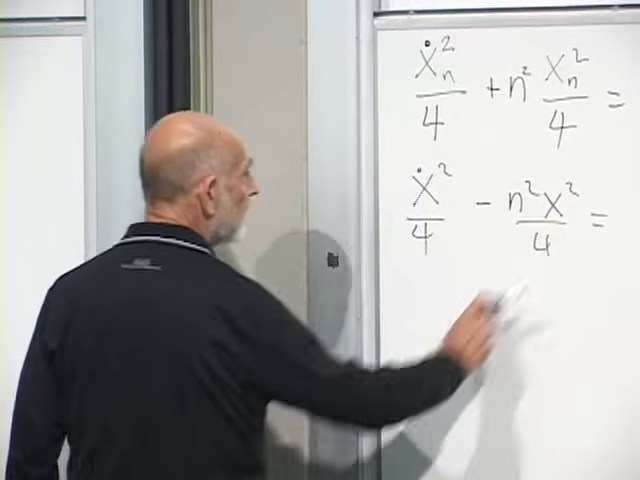
\includegraphics[width=0.82\textwidth]{lecture_03_figure_02.png}
  \caption{El cálculo en la pizarra muestra cómo el conmutador canónico aporta el factor de \(n\).}
  \lectureframe{00:10:30}
  \label{fig:l03-commutator-board}
\end{figure}

El factor de \(n\) nos indica cómo normalizar los operadores escalera:

\begin{align}
  a_n
  &\equiv
  \frac{\sqrt n}{2}X_n+\frac{i}{\sqrt n}p_n,
  \label{eq:l03-annihilator}\\
  a_n^\dagger
  &\equiv
  \frac{\sqrt n}{2}X_n-\frac{i}{\sqrt n}p_n.
  \label{eq:l03-creator}
\end{align}

Satisfacen

\begin{equation}
  [a_n,a_m^\dagger]=\delta_{nm},
  \qquad
  H_n=n\left(a_n^\dagger a_n+\frac12\right).
  \label{eq:l03-oscillator-algebra}
\end{equation}

Así, \(a_n^\dagger\) añade un cuanto del oscilador \(n\), pero ese cuanto lleva \(n\) unidades de energía del modo. No se pierde la separación habitual entre niveles del oscilador; su frecuencia es \(\omega_n=n\).

\begin{figure}[H]
  \centering
  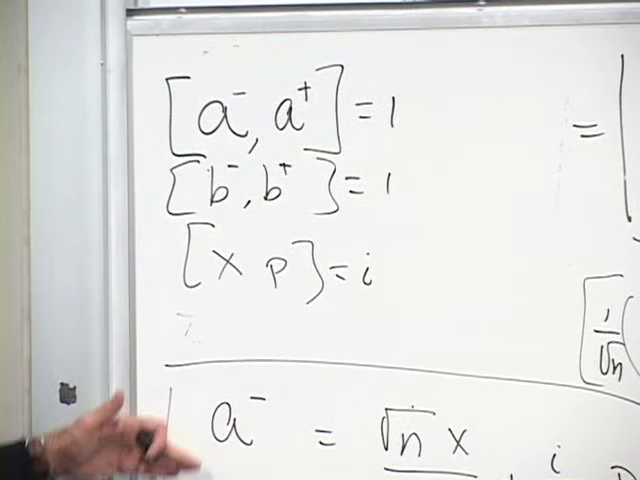
\includegraphics[width=0.82\textwidth]{lecture_03_figure_03.png}
  \caption{Operadores de aniquilación y creación normalizados para el oscilador de cuerda \(n\).}
  \lectureframe{00:12:00}
  \label{fig:l03-ladder-board}
\end{figure}

\subsection{Dos torres transversales}

En cuatro dimensiones espaciotemporales, una cuerda que lleva un momento muy grande a lo largo del eje \(z\) tiene dos coordenadas transversales, \(X\) y \(Y\). Por tanto, necesitamos dos torres independientes de osciladores. Sea \(a_n,a_n^\dagger\) el operador que actúa sobre los modos \(X\) y \(b_n,b_n^\dagger\) el que actúa sobre los modos \(Y\). Al despejar las coordenadas en \eqref{eq:l03-annihilator}--\eqref{eq:l03-creator}, obtenemos

\begin{equation}
  X_n=\frac{a_n+a_n^\dagger}{\sqrt n},
  \qquad
  Y_n=\frac{b_n+b_n^\dagger}{\sqrt n}.
  \label{eq:l03-mode-coordinates}
\end{equation}

\begin{figure}[H]
  \centering
  \includegraphics[width=0.78\textwidth]{lecture_03_figure_04.png}
  \caption{Despeje de la coordenada de un modo en función de sus operadores de creación y aniquilación.}
  \lectureframe{00:17:05}
  \label{fig:l03-coordinate-operator-board}
\end{figure}

Las coordenadas de la cuerda abierta se desarrollaron en modos de Neumann:

\begin{align}
  X(\sigma,\tau)
  &=X_{\rm cm}(\tau)
    +\sum_{n=1}^{\infty}X_n(\tau)\cos(n\sigma),
  \label{eq:l03-X-fourier}\\
  Y(\sigma,\tau)
  &=Y_{\rm cm}(\tau)
    +\sum_{n=1}^{\infty}Y_n(\tau)\cos(n\sigma).
  \label{eq:l03-Y-fourier}
\end{align}

Aparecen cosenos porque las pendientes en los extremos se anulan. Al sustituir \eqref{eq:l03-mode-coordinates}, la propia cuerda se convierte en un operador:

\begin{align}
  X(\sigma,\tau)
  &=X_{\rm cm}(\tau)
    +\sum_{n=1}^{\infty}
      \frac{a_n(\tau)+a_n^\dagger(\tau)}{\sqrt n}
      \cos(n\sigma),
  \label{eq:l03-X-operator}\\
  Y(\sigma,\tau)
  &=Y_{\rm cm}(\tau)
    +\sum_{n=1}^{\infty}
      \frac{b_n(\tau)+b_n^\dagger(\tau)}{\sqrt n}
      \cos(n\sigma).
  \label{eq:l03-Y-operator}
\end{align}

\begin{figure}[H]
  \centering
  \begin{minipage}[t]{0.48\textwidth}
    \centering
    \includegraphics[width=\textwidth]{lecture_03_figure_05.png}
    \par\smallskip\footnotesize (a) Desarrollos de las coordenadas en modos.
  \end{minipage}\hfill
  \begin{minipage}[t]{0.48\textwidth}
    \centering
    \includegraphics[width=\textwidth]{lecture_03_figure_06.png}
    \par\smallskip\footnotesize (b) Sustitución de los operadores escalera en las coordenadas de la cuerda.
  \end{minipage}
  \caption{La forma de la cuerda cuántica abierta se compone de todos sus operadores de oscilador transversales.}
  \lectureframe{00:20:35 and 00:21:05}
  \label{fig:l03-string-coordinate-board}
\end{figure}

\begin{classroomqa}
\audiencequestion{¿Es \(X_n\) también una función de \(\sigma\)?\lecturetimestamp{00:21:48}}
\lecturerresponse{No. Toda la dependencia de \(\sigma\) está en \(\cos(n\sigma)\). El coeficiente \(X_n\) es la amplitud, dependiente del tiempo, de ese patrón espacial, de modo que \(X_n=X_n(\tau)\).}
\end{classroomqa}

\begin{classroomqa}
\audiencequestion{¿Por qué los signos de los operadores llamados de subida y de bajada parecen estar invertidos?\lecturetimestamp{00:23:13}}
\lecturerresponse{El signo visible de \(ip_n\) no determina cómo se nombra el operador. Calculemos el conmutador con el hamiltoniano. El operador que satisface \([H_n,a_n^\dagger]=n a_n^\dagger\) aumenta la energía; el que satisface \([H_n,a_n]=-n a_n\) la disminuye.}
\end{classroomqa}

Las dos torres transversales son una representación pedagógica en cuatro dimensiones. Una cuerda bosónica cuantizada de forma consistente tiene veintiséis dimensiones espaciotemporales, por lo que posee veinticuatro familias de osciladores transversales en vez de dos. El razonamiento que sigue no cambia: el número de estados del primer nivel debe coincidir con el número de polarizaciones físicas de un vector sin masa en la misma dimensión.

\section{Espín masivo y helicidad sin masa}

Antes de asignar espín a los estados de la cuerda, necesitamos establecer una distinción clara. Una partícula masiva de espín \(J\) tiene \(2J+1\) estados de espín:

\begin{equation}
  m_J=-J,-J+1,\ldots,J-1,J.
  \label{eq:l03-massive-spin-multiplet}
\end{equation}

Por ejemplo, una partícula masiva de espín uno tiene tres polarizaciones y una partícula masiva de espín dos tiene cinco. Podemos ver por qué si pasamos al sistema de reposo. Allí están disponibles todas las rotaciones espaciales. Giramos el eje de espín y volvemos a transformar al sistema en movimiento: las \(2J+1\) componentes pertenecen a la misma partícula relativista.

Una partícula sin masa no tiene sistema de reposo. Su etiqueta invariante de espín es la helicidad, el momento angular en la dirección de su movimiento. El fotón solo tiene \(h=+1\) y \(h=-1\); el gravitón solo tiene \(h=+2\) y \(h=-2\). Un escalar tiene un único estado \(h=0\). En la clase se usa la simetría de reflexión para emparejar las dos helicidades. En una teoría quiral, una representación irreducible sin masa puede tener una sola helicidad, así que el emparejamiento es una afirmación adicional sobre la simetría, no una consecuencia de la ausencia de masa por sí sola.\editorialnote{La clasificación moderna mediante el grupo pequeño permite representaciones sin masa de una sola helicidad. La paridad o un contenido de campos que complete adecuadamente la simetría CPT aporta la helicidad opuesta en los ejemplos habituales del fotón y el gravitón.}

\begin{figure}[H]
  \centering
  \begin{minipage}[t]{0.45\textwidth}
    \centering
    \includegraphics[width=\textwidth]{lecture_03_figure_07.png}
    \par\smallskip\footnotesize (a) Recuento de estados de espín iniciado en la pizarra.
  \end{minipage}\hfill
  \begin{minipage}[t]{0.5\textwidth}
    \centering
    \begin{adjustbox}{max width=\linewidth}
    \begin{tabular}{@{}ccc@{}}
      \toprule
      Espín & Estados masivos & Hel icidades sin masa \\
      \midrule
      \(0\) & \(1\) & \(0\) \\
      \(1\) & \(3\) & \(+1,-1\) \\
      \(2\) & \(5\) & \(+2,-2\) \\
      \bottomrule
    \end{tabular}
    \end{adjustbox}
  \end{minipage}
  \caption{La masa elimina el sistema de reposo y, con él, las proyecciones intermedias del espín.}
  \lectureframe{00:27:40}
  \label{fig:l03-spin-count}
\end{figure}

\subsection{Polarización lineal y circular del fotón}

Consideremos un fotón que se mueve a lo largo de \(z\). Sus dos polarizaciones lineales transversales son \(\ket{x}\) y \(\ket{y}\). No son estados propios de helicidad. Los estados de polarización circular son

\begin{align}
  \ket{R}
  &=\frac{1}{\sqrt2}\left(\ket{x}+i\ket{y}\right),
  \label{eq:l03-right-circular}\\
  \ket{L}
  &=\frac{1}{\sqrt2}\left(\ket{x}-i\ket{y}\right),
  \label{eq:l03-left-circular}
\end{align}

con helicidades \(+1\) y \(-1\), según la convención usada para llamar derecha e izquierda a las polarizaciones. Un fotón con polarización lineal es una superposición de esos dos resultados. Su helicidad media puede anularse, pero una medición de helicidad nunca detecta un fotón de espín cero. Asimismo,

\begin{equation}
  \frac{1}{\sqrt2}\left(\ket{x}+\ket{y}\right)
\end{equation}

es simplemente una polarización lineal a cuarenta y cinco grados.

\begin{figure}[H]
  \centering
  \begin{minipage}[t]{0.48\textwidth}
    \centering
    \includegraphics[width=\textwidth]{lecture_03_figure_08.png}
    \par\smallskip\footnotesize (a) Estados de polarización circular en la pizarra.
  \end{minipage}\hfill
  \begin{minipage}[t]{0.48\textwidth}
    \centering
    \begin{adjustbox}{max width=\linewidth}
    \begin{tikzpicture}[>=Latex,scale=0.9]
      \draw[->,thick] (0,0) -- (3.4,0) node[right] {\(z\)};
      \draw[->,blue!70!black,thick] (0,0) -- (0,2.0)
        node[above] {\(x\)};
      \draw[->,orange!85!black,thick] (0,0) -- (-1.4,-1.2)
        node[below left] {\(y\)};
      \draw[red!70!black,thick,->]
        plot[domain=0:320,samples=80]
        ({1.0*cos(\x)},{0.58*sin(\x)+0.4});
      \node[red!70!black] at (1.55,1.25) {circular};
    \end{tikzpicture}
    \end{adjustbox}
  \end{minipage}
  \caption{La polarización lineal proporciona una base transversal; las combinaciones circulares diagonalizan la helicidad.}
  \lectureframe{00:37:45}
  \label{fig:l03-polarization}
\end{figure}

\begin{classroomqa}
\audiencequestion{¿Es esto parecido a la separación de estados de espín en un experimento de Stern--Gerlach?\lecturetimestamp{00:37:40}}
\lecturerresponse{La idea de superposición cuántica es la misma, pero para el fotón el término directo es polarización. Una medición de la polarización circular distingue las dos helicidades; en el haz no hay ningún fotón de espín cero con polarización longitudinal.}
\end{classroomqa}

El gravitón reproduce el patrón con espín dos. Para llevar la cuenta del espín, podemos escribir esquemáticamente

\begin{equation}
  \ket{+2}\sim\ket{+1}\otimes\ket{+1},
  \qquad
  \ket{-2}\sim\ket{-1}\otimes\ket{-1}.
  \label{eq:l03-graviton-helicity}
\end{equation}

Esto no significa que el gravitón esté literalmente compuesto por dos fotones. Significa que dos helicidades iguales se suman para dar la helicidad correcta de espín dos.

\begin{classroomqa}
\audiencequestion{¿La analogía con dos fotones se extiende a otros números cuánticos?\lecturetimestamp{00:41:05}}
\lecturerresponse{No como modelo de constituyentes. Hay fórmulas potentes en las que las amplitudes gravitatorias parecen productos, o ``cuadrados'', de amplitudes de teorías gauge, pero el gravitón sigue siendo una partícula propia. En este caso, la analogía resulta más fiable si se entiende como una afirmación sobre la helicidad.\editorialnote{Las relaciones de Kawai--Lewellen--Tye y las relaciones de doble copia precisan la afirmación sobre las amplitudes en teorías adecuadas; no convierten el gravitón en un estado ligado de dos fotones.}}
\end{classroomqa}

\begin{classroomqa}
\audiencequestion{Un fotón puede tener cualquier momento; ¿no tiene entonces un espectro continuo en vez del espectro discreto que se exige a una partícula?\lecturetimestamp{00:42:17}}
\lecturerresponse{La variable continua es el momento del centro de masas. Fijemos ese momento e inspeccionemos la masa invariante interna. Una partícula se identifica por un nivel de masa discreto; al variar luego su momento total se obtiene la relación de dispersión continua habitual.}
\end{classroomqa}

\section{Los niveles más bajos de la cuerda abierta}

Ahora podemos volver a la cuerda. En la descripción de momento grande, la energía interna finita de frente de luz es proporcional al cuadrado de la masa invariante. Omitiendo la escala global de la cuerda, escribimos el espectro así:

\begin{equation}
  \begin{aligned}
    M^2
    &=m_0^2
      +\sum_{n=1}^{\infty}n
       \left(N_n^{(a)}+N_n^{(b)}\right),\\
    N_n^{(a)}&=a_n^\dagger a_n,
    \qquad
    N_n^{(b)}=b_n^\dagger b_n.
  \end{aligned}
  \label{eq:l03-open-spectrum}
\end{equation}

El estado fundamental del oscilador satisface

\begin{equation}
  a_n\ket{0}=0,
  \qquad
  b_n\ket{0}=0,
  \qquad n=1,2,\ldots .
  \label{eq:l03-ground-annihilation}
\end{equation}

No es una ausencia de cuerda, sino la cuerda cuántica menos excitada, cuyas coordenadas siguen fluctuando. Sea \(m_0^2\) el cuadrado de su masa, aún por determinar.

\begin{figure}[H]
  \centering
  \includegraphics[width=0.78\textwidth]{lecture_03_figure_09.png}
  \caption{El estado fundamental de la cuerda abierta y las condiciones de aniquilación que lo definen.}
  \lectureframe{00:45:20}
  \label{fig:l03-ground-state-board}
\end{figure}

Las excitaciones de menor energía se obtienen usando los operadores de creación \(n=1\):

\begin{equation}
  a_1^\dagger\ket{0},
  \qquad
  b_1^\dagger\ket{0},
  \qquad
  M^2=m_0^2+1.
  \label{eq:l03-first-level}
\end{equation}

\begin{figure}[H]
  \centering
  \includegraphics[width=0.78\textwidth]{lecture_03_figure_10.png}
  \caption{Uno de los dos estados degenerados del primer nivel, con el incremento del cuadrado de la masa escrito en la pizarra.}
  \lectureframe{00:49:25}
  \label{fig:l03-first-level-board}
\end{figure}

El ``uno'' en eqref{eq:l03-first-level} no es un julio, un electronvoltio ni una masa de Planck. Hemos omitido la escala dimensional de cuerdas. Por ahora significa un peldaño en la escalera de masa al cuadrado del oscilador; las unidades que faltan se restablecerán en la próxima clase.

Cualquier combinación lineal de los dos estados degenerados también es un estado de este nivel. En particular,

\begin{equation}
  \frac{1}{\sqrt2}
  \left(a_1^\dagger\pm i b_1^\dagger\right)\ket{0}
  \label{eq:l03-string-circular-states}
\end{equation}

es el análogo de la polarización circular para la cuerda. Bajo una rotación en el plano \(x\)-\(y\), \(a_1^\dagger\) y \(b_1^\dagger\) se transforman como las dos componentes de un vector transversal. Las combinaciones de \eqref{eq:l03-string-circular-states} tienen, por tanto, helicidad \(+1\) y \(-1\).

\begin{figure}[H]
  \centering
  \includegraphics[width=0.82\textwidth]{lecture_03_figure_11.png}
  \caption{Las condiciones del estado fundamental, las dos excitaciones del primer nivel y sus combinaciones circulares, reunidas en la pizarra.}
  \lectureframe{00:56:00}
  \label{fig:l03-level-structure-board}
\end{figure}

No hay un tercer estado degenerado que pueda servir como polarización longitudinal. Si estos dos estados tuvieran masa distinta de cero, una partícula relativista de espín uno necesitaría tres polarizaciones. Al haber exactamente dos, el estado debe ser sin masa. Por tanto,

\begin{equation}
  m_0^2+1=0,
  \qquad
  m_0^2=-1.
  \label{eq:l03-intercept-condition}
\end{equation}

El primer nivel se parece a un fotón: es un estado vectorial gauge sin masa. No tiene por qué ser el fotón del electromagnetismo; su identidad gauge definitiva depende del modelo de cuerda. El estado fundamental que se encuentra por debajo tiene un cuadrado de la masa negativo. Es el taquión de la cuerda bosónica abierta.\editorialnote{En la cuerda bosónica crítica completa, el intercepto de orden normal y el álgebra de Lorentz están ligados a \(D=26\). El cálculo de la clase con dos direcciones transversales es la proyección en cuatro dimensiones del mismo argumento de recuento de estados: los estados de oscilador del primer nivel, \(D-2\), coinciden con las polarizaciones físicas \(D-2\) de un vector sin masa.}

\begin{classroomqa}
\audiencequestion{¿Por qué debería importarnos que \(m_0^2\) sea negativo?\lecturetimestamp{00:56:35}}
\lecturerresponse{Porque el cuadrado de la masa es la curvatura del potencial cuadrático del campo en torno al estado que hemos llamado vacío. Una curvatura negativa significa que esa configuración no es un estado fundamental estable. El siguiente cálculo precisa esta afirmación.}
\end{classroomqa}

\section{Qué significa realmente un taquión}

El nombre ``taquión'' invita a una primera interpretación engañosa. Partamos de la relación de dispersión relativista con \(c=1\):

\begin{equation}
  E(p)=\sqrt{p^2+m^2}.
  \label{eq:l03-relativistic-dispersion}
\end{equation}

Para un paquete de ondas, la velocidad de grupo es

\begin{equation}
  v_g=\frac{dE}{dp}.
  \label{eq:l03-group-velocity}
\end{equation}

Esto reproduce casos conocidos:

\begin{align}
  E_{\rm nr}(p)&=\frac{p^2}{2m},
  &v_g&=\frac{p}{m},
  \label{eq:l03-nr-group-velocity}\\
  E_\gamma(p)&=|p|,
  &|v_g|&=1,
  \label{eq:l03-photon-group-velocity}\\
  E_m(p)&=\sqrt{p^2+m^2},
  &|v_g|&=\frac{|p|}{\sqrt{p^2+m^2}}<1.
  \label{eq:l03-massive-group-velocity}
\end{align}

\begin{figure}[H]
  \centering
  \begin{minipage}[t]{0.48\textwidth}
    \centering
    \includegraphics[width=\textwidth]{lecture_03_figure_12.png}
    \par\smallskip\footnotesize (a) Velocidad de grupo no relativista.
  \end{minipage}\hfill
  \begin{minipage}[t]{0.48\textwidth}
    \centering
    \includegraphics[width=\textwidth]{lecture_03_figure_13.png}
    \par\smallskip\footnotesize (b) Dispersión relativista y su derivada.
  \end{minipage}
  \caption{Obtención de la velocidad de propagación a partir de la pendiente de \(E(p)\).}
  \lectureframe{01:01:50 and 01:03:15}
  \label{fig:l03-group-velocity-board}
\end{figure}

Si \(m^2=-\mu^2\), la expresión formal queda

\begin{equation}
  E(p)=\sqrt{p^2-\mu^2},
  \qquad
  v_g=\frac{p}{\sqrt{p^2-\mu^2}},
  \label{eq:l03-formal-tachyon-dispersion}
\end{equation}

que satisface \(|v_g|>1\) siempre que la raíz cuadrada sea real. Pero esta no es la interpretación física correcta del estado fundamental de la cuerda bosónica. El problema ya aparece a bajo momento, donde la frecuencia es imaginaria.

\subsection{Curvatura negativa del potencial del campo}

Consideremos un campo escalar real en una dimensión espacial:

\begin{equation}
  \left(\partial_t^2-\partial_x^2+m^2\right)\phi=0.
  \label{eq:l03-klein-gordon}
\end{equation}

Para una onda plana \(\phi\propto e^{-i\omega t+ikx}\),

\begin{equation}
  \omega^2=k^2+m^2.
  \label{eq:l03-kg-dispersion}
\end{equation}

\begin{figure}[H]
  \centering
  \includegraphics[width=0.82\textwidth]{lecture_03_figure_14.png}
  \caption{La ecuación de Klein--Gordon usada para poner de manifiesto la inestabilidad que subyace al cuadrado de la masa negativo.}
  \lectureframe{01:06:40}
  \label{fig:l03-klein-gordon-board}
\end{figure}

La energía cuadrática conservada es

\begin{equation}
  \mathcal E
  =\frac12\int dx\,
  \left[
    \dot\phi^{\,2}
    +(\partial_x\phi)^2
    +m^2\phi^2
  \right].
  \label{eq:l03-field-energy}
\end{equation}

\begin{figure}[H]
  \centering
  \includegraphics[width=0.82\textwidth]{lecture_03_figure_15.png}
  \caption{La energía del campo escalar, donde el término de masa determina la curvatura local del potencial.}
  \lectureframe{01:08:10}
  \label{fig:l03-field-energy-board}
\end{figure}

Para \(m^2>0\), el potencial local \(V(\phi)=\tfrac12m^2\phi^2\) tiene forma de cuenco. La configuración \(\phi=0\) está en el fondo. Para \(m^2=-\mu^2\), ese mismo punto se encuentra en la cima de un cuenco invertido. La ecuación \eqref{eq:l03-kg-dispersion} se convierte en

\begin{equation}
  \omega^2=k^2-\mu^2.
  \label{eq:l03-tachyonic-modes}
\end{equation}

Los modos con \(k^2<\mu^2\) tienen

\begin{equation}
  \omega=\pm i\sqrt{\mu^2-k^2},
  \qquad
  \phi_k(t)\propto
  e^{\pm\sqrt{\mu^2-k^2}\,t}.
  \label{eq:l03-growing-mode}
\end{equation}

Una de las ramas crece exponencialmente. Por tanto, el supuesto vacío es inestable: una perturbación de longitud de onda grande, por pequeña que sea, aleja el campo de \(\phi=0\). Eso es lo que significa que haya un taquión en el espectro.

\subsection{La secuencia del péndulo invertido}

Una hilera de péndulos acoplados permite ver la distinción. Coloquemos todos los péndulos en posición vertical. La configuración uniforme existe, pero está en equilibrio en un máximo de energía potencial. Si empujamos un péndulo, cae y tira de sus vecinos. Un frente de péndulos que caen se propaga por la hilera a la velocidad finita de señal que fijan los acoplamientos.

\begin{figure}[H]
  \centering
  \begin{minipage}[t]{0.48\textwidth}
    \centering
    \includegraphics[width=\textwidth]{lecture_03_figure_16.png}
    \par\smallskip\footnotesize (a) El modelo de péndulos verticales acoplados de la pizarra.
  \end{minipage}\hfill
  \begin{minipage}[t]{0.48\textwidth}
    \centering
    \begin{adjustbox}{max width=\linewidth}
    \begin{tikzpicture}[>=Latex,scale=0.78]
      \draw[thick] (-0.3,0) -- (6.3,0);
      \foreach \x/\a in {0/0,1/0,2/8,3/28,4/55,5/72,6/78}{
        \fill (\x,0) circle (0.06);
        \draw[thick] (\x,0) -- ++({90-\a}:1.25);
        \fill[blue!65!black]
          ($(\x,0)+({90-\a}:1.25)$) circle (0.11);
      }
      \draw[red!70!black,->,thick] (1.7,-0.45) -- (4.6,-0.45)
        node[midway,below] {falling front};
    \end{tikzpicture}
    \end{adjustbox}
  \end{minipage}
  \caption{La inestabilidad se propaga causalmente por un sistema aunque su espectro linealizado contenga un cuadrado de la masa negativo.}
  \lectureframe{01:10:40}
  \label{fig:l03-pendulum-instability}
\end{figure}

Nada en este mecanismo permite que una señal controlada se adelante al frente causal. Un modo taquiónico revela un punto de expansión inadecuado, no un mensajero superlumínico estable.\editorialnote{En una ecuación de campo relativista local, la velocidad del frente sigue siendo la velocidad causal. La velocidad de grupo formal de la rama real a alta \(k\) no convierte el vacío inestable en un canal de comunicación más rápido que la luz.}

\begin{classroomqa}¿Es el estado sin masa que acabamos de encontrar el gravitón que predice la teoría de cuerdas?\audiencequestion{\lecturetimestamp{01:14:27}}
\lecturerresponse{No. Es el estado de espín uno de una cuerda abierta con dos polarizaciones, por lo que se parece a un bosón gauge. El gravitón es una excitación de espín dos de una cuerda cerrada.}
\end{classroomqa}

\begin{classroomqa}¿Es matemáticamente admisible un potencial invertido y dónde acabaría el sistema después de caer?\audiencequestion{\lecturetimestamp{01:15:17}}
\lecturerresponse{Es una aproximación local perfectamente legítima, pero por sí sola no tiene estado fundamental porque la energía no está acotada inferiormente. Un potencial más completo puede volver a curvarse hacia arriba y tener un mínimo más bajo. Entonces el sistema rueda o condensa hacia esa configuración estable.}
\end{classroomqa}

La cuerda bosónica ordinaria tiene precisamente este defecto. Sus estados de oscilador de mayor energía siguen formando parte del espectro, pero son excitaciones de un fondo inestable. Las teorías de supercuerdas consistentes eliminan el taquión de cuerda abierta en sus sectores estables, a la vez que conservan excitaciones de cuerda sin masa y masivas.

\begin{classroomqa}¿Las demás propiedades del estado de cuerda abierta coinciden con las de un fotón tanto como coinciden sus dos polarizaciones?\audiencequestion{\lecturetimestamp{01:17:07}}
\lecturerresponse{El estado se comporta como un bosón gauge sin masa. Sus asignaciones de carga, reglas de radiación e identidad detalladas dependen del modelo de cuerda, así que conviene llamarlo parecido a un fotón en vez de identificarlo de inmediato con el electromagnetismo. Las interacciones correspondientes se desarrollarán más adelante.}
\end{classroomqa}

\section{Cómo interactúan las cuerdas}

El espectro libre es solo la mitad de la teoría. Las cuerdas también se unen y se dividen. Conviene recordar primero que una cuerda libre excitada puede llevar momento angular. Una cuerda recta en rotación gira alrededor de su centro de masas, y su energía y su momento angular aumentan juntos siguiendo la trayectoria característica de las cuerdas.

\begin{figure}[H]
  \centering
  \includegraphics[width=0.72\textwidth]{lecture_03_figure_17.png}
  \caption{Esquema de una cuerda abierta que gira alrededor de su centro de masas.}
  \lectureframe{01:19:30}
  \label{fig:l03-rotating-string-board}
\end{figure}

\begin{classroomqa}¿Puede una cuerda libre girar de extremo a extremo alrededor de un extremo fijo?\audiencequestion{\lecturetimestamp{01:20:02}}
\lecturerresponse{No, si no está anclada. Un sistema libre y aislado gira alrededor de su centro de masas. Si un extremo está unido a otro objeto o a una brana, el sistema conjunto puede girar alrededor de otro centro, igual que un electrón y un núcleo orbitan en torno a su centro de masas común mientras el núcleo, mucho más pesado, parece casi inmóvil.}
\end{classroomqa}

\subsection{El vértice de cuerda abierta}

En las cuerdas abiertas, la interacción elemental ocurre cuando dos extremos coinciden en el mismo punto del espacio-tiempo. Hay una amplitud \(g_s\) para que se unan y formen una sola cuerda. Si invertimos la evolución, obtenemos una amplitud para que una cuerda se divida en dos. Esquemáticamente:

\begin{equation}
  \text{open}+\text{open}
  \quad\rightleftarrows\quad
  \text{open}.
  \label{eq:l03-open-joining}
\end{equation}

\begin{figure}[H]
  \centering
  \begin{minipage}[t]{0.48\textwidth}
    \centering
    \includegraphics[width=\textwidth]{lecture_03_figure_18.png}
    \par\smallskip\footnotesize (a) La evolución de unión en la pizarra.
  \end{minipage}\hfill
  \begin{minipage}[t]{0.48\textwidth}
    \centering
    \begin{tikzpicture}[>=Latex,scale=0.9]
      \draw[->] (0,-2.1) -- (0,2.2) node[above] {time};
      \draw[blue!70!black,thick] (-2,-1.6) .. controls (-1.3,-0.9)
        and (-0.7,-0.35) .. (0,0);
      \draw[blue!70!black,thick] (2,-1.6) .. controls (1.3,-0.9)
        and (0.7,-0.35) .. (0,0);
      \draw[orange!85!black,thick] (0,0) .. controls (0.25,0.7)
        and (-0.15,1.25) .. (0.15,1.9);
      \fill[red!70!black] (0,0) circle (0.09);
      \node[right] at (0.12,0) {\(g_s\)};
    \end{tikzpicture}
  \end{minipage}
  \caption{La unión de extremos es el análogo, para las cuerdas, de un vértice de interacción local entre partículas; la inversión temporal da la división.}
  \lectureframe{01:24:05}
  \label{fig:l03-open-vertex}
\end{figure}

El acoplamiento es una amplitud. Para un proceso elemental especificado, la probabilidad correspondiente comienza en el orden \(|g_s|^2\), con factores de espacio de fases y de normalización que aporta el cálculo completo. Llamar \(g_s\)``probabilidad'' al acoplamiento es, por tanto, una forma abreviada e informal de expresarse; distinguir entre amplitud y probabilidad evita introducir un cuadrado espurio.

La interacción no depende de si la cuerda externa está vibrando, girando o en algún otro estado de oscilador. Esos estados modifican el elemento de matriz detallado, pero se aplica la misma regla local de unión.

\subsection{Una cuerda abierta puede cerrarse sobre sí misma}

Supongamos que se encuentran los dos extremos de una cuerda abierta. La regla de unión no puede saber que pertenecen a la misma cuerda. Pueden fusionarse y formar un lazo cerrado:

\begin{equation}
  \text{open}\longrightarrow\text{closed}.
  \label{eq:l03-self-closing}
\end{equation}

\begin{figure}[H]
  \centering
  \begin{minipage}[t]{0.48\textwidth}
    \centering
    \includegraphics[width=\textwidth]{lecture_03_figure_19.png}
    \par\smallskip\footnotesize (a) La cuerda abierta acerca sus extremos.
  \end{minipage}\hfill
  \begin{minipage}[t]{0.48\textwidth}
    \centering
    \begin{tikzpicture}[>=Latex,scale=0.92]
      \draw[blue!70!black,thick]
        (-2,0) .. controls (-1.2,1.5) and (1.2,1.5) .. (2,0);
      \fill[red!70!black] (-2,0) circle (0.08);
      \fill[red!70!black] (2,0) circle (0.08);
      \draw[->,thick] (-0.45,-0.45) -- (0.45,-0.45);
      \draw[orange!85!black,thick] (0,-1.55) ellipse (1.15 and 0.58);
      \node at (0,-2.25) {closed string};
    \end{tikzpicture}
  \end{minipage}
  \caption{Las cuerdas abiertas que interactúan generan inevitablemente cuerdas cerradas.}
  \lectureframe{01:27:20}
  \label{fig:l03-open-becomes-closed}
\end{figure}

Esto no es un añadido opcional. Toda teoría de cuerdas abiertas que interactúan debe contener estados de cuerda cerrada. El proceso inverso permite que una cuerda cerrada se abra y se convierta en una cuerda abierta cuando las condiciones de contorno y los extremos permitidos lo admiten.

\begin{classroomqa}Cuando las cuerdas se fusionan o se dividen, ¿cambia su energía de oscilación y determina la teoría cómo ocurre?\audiencequestion{\lecturetimestamp{01:28:05}}
\lecturerresponse{Sí. La energía y el momento se conservan en el proceso completo, mientras que la excitación puede redistribuirse entre las cuerdas salientes. El vértice de interacción y las funciones de onda externas determinan la amplitud de transición.}
\end{classroomqa}

\subsection{Las cuerdas cerradas pueden interactuar sin abrirse}

La implicación es unidireccional. Las cuerdas abiertas que interactúan requieren cuerdas cerradas, pero una teoría puede comenzar solo con cuerdas cerradas. Dos lazos cerrados pueden tocarse, reconectarse y convertirse en un solo lazo cerrado; la evolución inversa divide un lazo en dos. No es necesario que aparezca ningún extremo abierto.

\begin{figure}[H]
  \centering
  \begin{minipage}[t]{0.48\textwidth}
    \centering
    \includegraphics[width=\textwidth]{lecture_03_figure_20.png}
    \par\smallskip\footnotesize (a) Fusión de cuerdas cerradas en la pizarra.
  \end{minipage}\hfill
  \begin{minipage}[t]{0.48\textwidth}
    \centering
    \begin{tikzpicture}[>=Latex,scale=0.88]
      \draw[blue!70!black,thick] (-1.35,0) circle (0.75);
      \draw[blue!70!black,thick] (1.35,0) circle (0.75);
      \draw[->,thick] (-0.35,-1.15) -- (0.35,-1.15);
      \draw[orange!85!black,thick] (0,-2.3) ellipse (1.35 and 0.68);
      \node at (0,1.2) {closed \(+\) closed};
      \node at (0,-3.25) {closed};
    \end{tikzpicture}
  \end{minipage}
  \caption{Las cuerdas cerradas tienen su propia interacción de unión y división y no necesitan pasar por un estado de cuerda abierta.}
  \lectureframe{01:29:05}
  \label{fig:l03-closed-fusion}
\end{figure}

\begin{classroomqa}Si una teoría comienza con cuerdas cerradas, ¿debe contener también cuerdas abiertas?\audiencequestion{\lecturetimestamp{01:28:35}}
\lecturerresponse{No. Las cuerdas cerradas pueden interactuar mediante reconexión y seguir siendo cerradas en todo momento. Las cuerdas abiertas requieren datos de contorno adicionales, como extremos permitidos o branas.}
\end{classroomqa}

\section{Por qué no se puede evitar la gravedad}

El cálculo de los osciladores de la cuerda cerrada es análogo al de la cuerda abierta, pero hay excitaciones independientes que se mueven a izquierda y a derecha. Su primer nivel no trivial con niveles coincidentes contiene un estado sin masa de espín dos. Ese estado tiene las helicidades de un gravitón. Por consiguiente, toda teoría consistente de cuerdas cerradas contiene gravedad.

\begin{classroomqa}
\audiencequestion{¿Por qué la excitación de menor energía de la cuerda cerrada tiene que ser un gravitón, igual que el nivel de la cuerda abierta tenía que ser de tipo fotónico?
\lecturetimestamp{01:30:59}}
\lecturerresponse{La respuesta se basa en el mismo tipo de conteo de estados, ahora con vectores de oscilador de movimiento hacia la izquierda y hacia la derecha. Su producto tensorial contiene una polarización sin masa, simétrica, sin traza y de espín dos. El espectro explícito de la cuerda cerrada se desarrollará en la próxima clase; en esta etapa, lo esencial es que ese estado es inevitable.}
\end{classroomqa}

Las cuerdas abiertas y cerradas también pueden interactuar entre sí. Un lazo cerrado puede encontrarse con una cuerda abierta y ser absorbido, dejando una cuerda abierta más larga o con una excitación distinta. A la inversa, una cuerda abierta puede emitir un lazo cerrado. En términos de partículas, esto corresponde a la emisión o absorción de un gravitón por la materia.

\begin{figure}[H]\centering
  \begin{minipage}[t]{0.48\textwidth}
    \centering
    \includegraphics[width=\textwidth]{lecture_03_figure_21.png}
    \par\smallskip\footnotesize (a) Reconexión local de segmentos de cuerda.
  \end{minipage}\hfill
  \begin{minipage}[t]{0.48\textwidth}
    \centering
    \includegraphics[width=\textwidth]{lecture_03_figure_22.png}
    \par\smallskip\footnotesize (b) Un lazo cerrado se une a una cuerda abierta.
  \end{minipage}
  \caption{Los esquemas de la pizarra ilustran las interacciones entre cuerdas abiertas--y cerradas, así como la posibilidad universal de intercambiar gravitones.}
  \lectureframe{01:33:10 and 01:34:35}
  \label{fig:l03-mixed-interactions-board}
\end{figure}

\begin{figure}[H]
  \centering
  \begin{tikzpicture}[>=Latex,scale=0.88]
    \draw[blue!70!black,thick]
      (-3,-0.5) .. controls (-1.7,-0.1) and (-0.8,0.2) .. (0,0);
    \draw[blue!70!black,thick]
      (0,0) .. controls (0.9,0.3) and (2.0,0.1) .. (3,0.55);
    \draw[orange!85!black,thick] (-0.8,1.55) ellipse (0.75 and 0.45);
    \draw[->,red!70!black,thick] (-0.45,1.15) -- (-0.05,0.35);
    \node[blue!70!black] at (-2.2,-0.95) {open string};
    \node[orange!85!black] at (-0.8,2.25) {closed string};
    \node at (1.75,-0.5) {excited open string};
  \end{tikzpicture}
  \caption{Esquema nítido, sin representación del espacio-tiempo, de la absorción de una cuerda cerrada por una cuerda abierta.}
  \label{fig:l03-mixed-interaction-redraw}
\end{figure}

El gravitón puede acoplarse a todos los estados de cuerda porque toda cuerda lleva energía y momento, y las reglas de unión permiten intercambiar cuerdas cerradas. Este es el origen, en la teoría de cuerdas, de la universalidad de la gravedad.

\begin{classroomqa}\audiencequestion{¿Puede una cuerda cerrada convertirse en abierta, o unirse a una cuerda abierta sin violar la regla de los extremos?\lecturetimestamp{01:31:20}}
\lecturerresponse{En una teoría que contenga ambos sectores, una cuerda cerrada puede unirse a una abierta y cambiar su estado. Que una cuerda cerrada aislada pueda simplemente abrirse depende de que la teoría permita extremos admisibles. La regla local de reconexión sigue siendo la misma.}
\end{classroomqa}

\begin{classroomqa}
\audiencequestion{¿Pueden los lazos cerrados quedar enlazados o anudados de forma permanente?\lecturetimestamp{01:35:10}}
\lecturerresponse{A acoplamiento débil, las cuerdas son casi siempre transparentes: pueden atravesarse unas a otras, salvo cuando actúa la pequeña amplitud de reconexión. Por tanto, un enlace o un nudo puede persistir durante algún tiempo, pero la topología puede cambiar cuando se produce una interacción permitida entre cuerdas.}
\end{classroomqa}

\begin{classroomqa}
\audiencequestion{¿La probabilidad de interacción es independiente del estado o la velocidad de la cuerda?\lecturetimestamp{01:36:09}}
\lecturerresponse{El acoplamiento local es el mismo parámetro, pero la probabilidad total de transición también depende de las funciones de onda y del tiempo que las partes pertinentes permanezcan en contacto. Por lo general, un encuentro rápido ofrece menos tiempo para la interacción que uno lento.}
\end{classroomqa}

\section{La escala y el acoplamiento que aún faltan}

Se han dejado deliberadamente para más adelante dos cuestiones de contabilidad. En primer lugar, \(X\) es una longitud, mientras que \(a_n\) es adimensional, así que la proporcionalidad de \eqref{eq:l03-mode-coordinates} debe incluir una escala de longitud. En segundo lugar, elevar el nivel del oscilador no puede añadir literalmente un número adimensional a una masa física al cuadrado. Al recuperar la longitud de cuerda \(\ell_s\), o, de manera equivalente, la pendiente de Regge \(\alpha'\sim\ell_s^2\), se obtienen las dimensiones que faltan:

\begin{equation}
  M^2\sim\frac{1}{\alpha'}(N-a).
  \label{eq:l03-dimensional-spectrum}
\end{equation}

La convención y la normalización precisas se establecerán en la próxima clase.

\begin{classroomqa}
\audiencequestion{¿Qué determina la unidad de longitud de cuerda y la masa que aporta cada operador de creación?\lecturetimestamp{01:37:03}}
\lecturerresponse{Se ha suprimido una constante dimensional: la escala de cuerda, que suele denotarse por \(\ell_s\) o \(\alpha'\). Los operadores osciladores son adimensionales; las potencias de esa escala convierten el número de nivel en longitud, tensión y masa al cuadrado físicas.}
\end{classroomqa}

El segundo parámetro es el acoplamiento de cuerda \(g_s\). En el tratamiento más sencillo, es un número universal que controla la unión y la separación de cuerdas. En modelos más ricos, los extremos pueden llevar etiquetas distintas y las cuerdas pueden encontrarse en uniones. Una configuración en forma de Y es el análogo, para cuerdas, de tres tubos de flujo que se encuentran; en la antigua imagen hadrónica se asocia con un barión de tres quarks, mientras que un único segmento abierto se asemeja a un mesón de quark--antiquark.

\begin{classroomqa}
\audiencequestion{¿Pueden tener los extremos de distintas cuerdas probabilidades de unión diferentes?\lecturetimestamp{01:39:31}}
\lecturerresponse{El modelo más sencillo utiliza un solo acoplamiento. Las teorías más elaboradas asignan cargas o etiquetas de contorno a los extremos, y las reglas de selección determinan entonces qué uniones están permitidas. La construcción detallada se verá más adelante, pero la idea universal de unión local se mantiene.}
\end{classroomqa}

\begin{classroomqa}
\audiencequestion{¿Puede una cuerda dividirse a lo largo o formar una unión en Y?\lecturetimestamp{01:40:01}}
\lecturerresponse{Algunos sistemas de cuerdas sí admiten uniones. No se trata del proceso ordinario de división de una cuerda con dos extremos que acabamos de dibujar, sino de uniones que aparecen cuando la teoría admite cargas de cuerda compatibles. La analogía entre el tubo de flujo del mesón-- y el del barión es una imagen útil para entender la distinción.}
\end{classroomqa}

\begin{classroomqa}
\audiencequestion{¿Cambiar el número de dimensiones del espacio-tiempo modifica el acoplamiento de interacción?\lecturetimestamp{01:42:25}}
\lecturerresponse{Las dimensiones modifican el espectro, el espacio de fases y los acoplamientos efectivos que se obtienen tras la compactificación. El acoplamiento fundamental de cuerda sigue organizando la expansión perturbativa, pero su manifestación en menos dimensiones depende de la geometría y el volumen de las dimensiones extra.}
\end{classroomqa}

\begin{classroomqa}
\audiencequestion{¿Es la gravedad lo que hace que una cuerda libre se mueva desde el principio?\lecturetimestamp{01:43:17}}
\lecturerresponse{No hace falta ninguna fuerza para mantener el movimiento. La posición y la velocidad iniciales especifican una solución libre; la inercia la mantiene en movimiento. La gravedad u otra fuerza modifica ese movimiento. Preguntar qué causó las condiciones iniciales es una cuestión aparte, ajena a la ecuación local de movimiento.}
\end{classroomqa}

Hemos llegado, por tanto, a tres conclusiones relacionadas. La cuantización de una cuerda abierta produce un vector sin masa en su primer nivel excitado; el estado fundamental bosónico que está por debajo es inestable; y las interacciones introducen inevitablemente cuerdas cerradas, cuyo espectro contiene la gravedad. La siguiente tarea consiste en recuperar la escala que falta y llevar a cabo explícitamente la cuantización de la cuerda cerrada.